\chapter{Ejemplo de ap\'{e}ndice: El problema de la medida}\label{C:ap1}
\chapterquote{Que miseria che, tres empanadas}{Brandoni, 2018}
\graphicspath{{figs/}}
%%%%%%%%%%%%%%%%%%%%%%%%%%%%%%%%%%%%%%%%%%%%%%%%%%%%%%%%%%%%%%%%%%%%%%%%
Una figura en el apendice se ve así,
\begin{figure}[ht]
\centering{}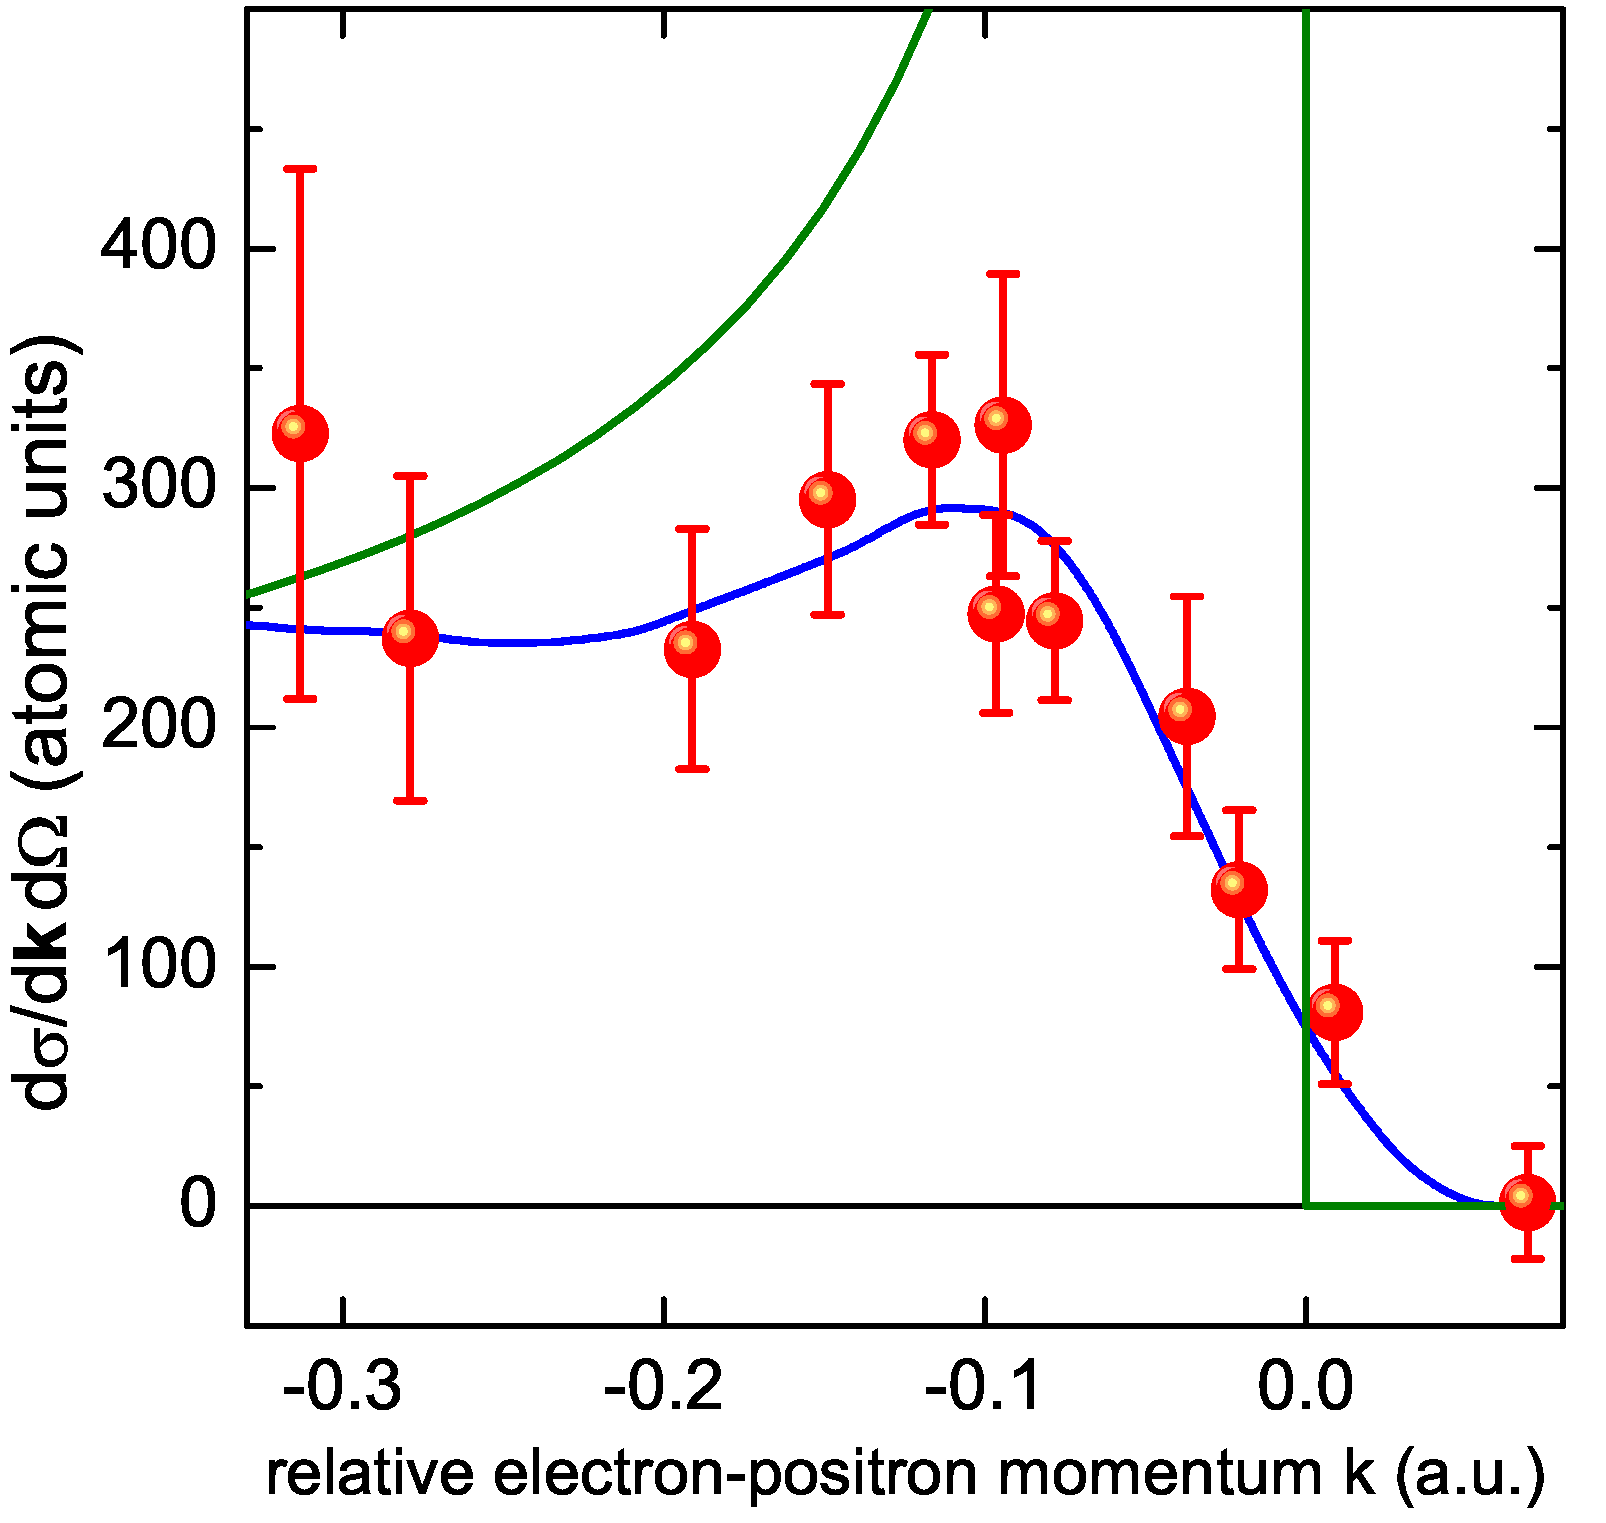
\includegraphics[width=\imsize]{ap1_f1}
\caption{Una figura con algunos puntos experimentales y curva de datos te\'{o}ricos\label{f:figura1}}  
\end{figure}

%%% Local Variables: 
%%% mode: latex
%%% TeX-master: "main"
%%% End: 
